\documentclass[a4paper,12pt]{article}

% packages and main settings
\usepackage{booktabs}
\usepackage[left=3cm, right=2cm, top=2cm, bottom=2cm]{geometry}
\usepackage[english]{babel}
\usepackage[utf8]{inputenc}
\usepackage[T1]{fontenc}
\usepackage{lmodern}
\usepackage{microtype}
\usepackage{amsmath}
\usepackage{amsfonts, amsthm, amssymb, graphicx, booktabs}
\usepackage[ruled,vlined]{algorithm2e}
\usepackage{bm} %bold epsilon
\usepackage{newclude}
\usepackage{placeins}  %surpresses floating tables
\usepackage[labelfont=bf]{caption} %Figure etc steht dann in small caps
\usepackage[labelsep=period]{caption} % dot after figure, table caption.
\usepackage[flushleft]{threeparttable} % for notes below table
\usepackage{multirow} % for table cell merge along rows
\usepackage{graphicx} % to adjust tablesize to textwidth
\usepackage{caption}  % for centered captions
\usepackage{float} % to set of autopositioning of tables
\usepackage[bottom,hang,flushmargin]{footmisc} % forces footnotes to the bottom
\usepackage{setspace}           % Fuer 1.5 fachen Zeilenabstand
\onehalfspacing % 1.5 cm Zeilenabstand
%Bibtex
\usepackage[round,sort&compress]{natbib}

\bibliographystyle{chicago} % chicago bib style like in AER
\usepackage[hidelinks]{hyperref} % fuer links und verweise. Cleverref ist eigentlich besser.
\usepackage{subfig}


% Create header. The header must be surpressed for
% every first page per section and a solution
% for the Appendix is used in the respective subfile.
\usepackage{fancyhdr}
\pagestyle{fancy}
\fancyhf{}
\chead{\nouppercase{\textit{\leftmark}}}
\cfoot{\thepage}
\renewcommand{\headrulewidth}{0pt} % no vertical line

%\usepackage{lipsum}  % check if formats work

\usepackage{afterpage} %clearpage w/o pagebreak for "header bug"

% Expectation symbol
\DeclareMathOperator*{\E}{\mathbb{E}}


% for strike through
\DeclareMathOperator*{\argmax}{argmax}
\newcommand*{\defeq}{\stackrel{\text{def}}{=}}
\usepackage[normalem]{ulem}
% try to use strikeout in section headers and others
\DeclareRobustCommand{\hsout}[1]{\texorpdfstring{\sout{#1}}{#1}}

% for gray table row color
\usepackage[table]{xcolor}

% decimal dot alignment in table columns
\usepackage{siunitx}

% for footnotes in table
\usepackage[flushleft]{threeparttable}

% for underbar
\newcommand{\ubar}[1]{\text{\b{$#1$}}}

\usepackage{tikz}

% Setup for urls
\usepackage{url}


%Steps list
\usepackage{enumitem}

% indented multirow captions.
\usepackage{caption}



\begin{document}


\begin{titlepage}
	
\begin{center}
	
\vspace*{1.0cm}

{\LARGE
\bfseries Mathematical Programming with Equilibrium Constraints: \\
\vspace*{0.5cm}
An Uncertainty Perspective
}
\\


{\large
\vspace*{4.0cm}
Master Thesis Presented to the\\
\vspace*{0.25cm}
Department of Economics at the\\
\vspace*{0.25cm}
Rheinische Friedrich-Wilhelms-Universität Bonn\\

\vspace*{2.0cm}
in Partial Fulfillment of the Requirements for the Degree of\\
\vspace*{0.25cm}
Master of Science (M.Sc.)\\

\vspace*{4.0cm}
Supervisor: Prof. Dr. Philipp Eisenhauer\\

\vspace*{2.0cm}
Submitted in August 2020 by:\\
Pascal Heid\\
Matriculation Number: 3220685
}

\end{center}

\end{titlepage}

\newpage

\thispagestyle{plain} % no header on first page
\tableofcontents
\newpage

\setcounter{page}{1}
\pagenumbering{Roman}


% no section command to prevent "A" before "Appendix" in toc.

\addcontentsline{toc}{section}{Abbreviations} 

\section*{Abbreviations} % no number before Appendix in toc
\thispagestyle{plain} % surpress header on first page

\phantom{This text will be invisible} 
\hspace{20cm}



% Please add the following required packages to your document preamble:
% \usepackage{booktabs}
\begin{table}[H]
	\centering
	\renewcommand{\arraystretch}{1.2}%
	\begin{tabular}{@{}ll@{}}
		\toprule
	Term\phantom{space}	& Meaning \\ \midrule
		$\bold{VI}$	& Variational Inequality \\
		$\bold{NFXP}$	& Nested Fixed Point Algorithm \\
		$\bold{MPEC}$	& Mathematical Programming with Equilibrium Constraints \\
		$\bold{N-K}$	& Newton-Kantorovich \\
 \bottomrule
	\end{tabular}
\end{table}
\newpage
\addcontentsline{toc}{section}{List of Figures}

%\section*{List of Figures} % no number before LoFs in toc
\thispagestyle{plain} % surpress header on first page

\listoffigures
\newpage
\addcontentsline{toc}{section}{List of Tables}

%\section*{List of Tables} % no number before LoTs in toc
\thispagestyle{plain} % surpress header on first page

\listoftables
\newpage
\addcontentsline{toc}{section}{List of Algorithms} 

%\section*{List of Figures} % no number before LoFs in toc
\thispagestyle{plain} % surpress header on first page

\listofalgorithms
\addtocontents{loa}{\def\string\figurename{Algorithm}}
\newpage

\setcounter{page}{1}
\pagenumbering{arabic}

%\section{Introduction}
\thispagestyle{plain} % surpress header on first page


%\afterpage{\clearpage} % solves problem that header does not disappear in
% literature review
\section{Mathematical Programming with Equilibrium Constraints}
\thispagestyle{plain} % surpress header on first page

Mathematical Programming with Equilibrium Constraints can be traced back notation and concept wise to Game Theory. Specifically in the theory on Stackelberg games MPEC found its first development. It was due to \cite{Luo.Pang.Ralph.1996}, though, that MPEC was set onto a mathematically rigorous foundation. They argue to have done so in order to present its manifold possibilities of application that had been overlooked previously. 

Before we go into the details of MPEC regarding its mathematical formulation, applications and use in Economics, let us break down the lengthy term into its key components. The beginning "Mathematical Program" solely captures that we look at a mathematical optimization problem. The particularity of this problem comes in with the "Equilibrium Constraints". Mathematically this means that this optimization problem is subject to variational inequalities (VI) as constraints. \cite{Nagurney.1993} explains that VIs consist of but are not limited to nonlinear equations, optimization as well as fixed point problems. More broadly spoken VIs are able to harnesses our intuitive notion of economic equilibrium for which typically a functional or a system of equations must be solved for all possible values of a given input. This is tightly linked to what is looked for when solving a Stackelberg game. Essentially, an economic equilibrium has to be found. As a reminder in a Stackelberg game, there is one leader that moves first followed by the moves of some followers. Solving this problem involves the leader to solve an optimization problem that in turn is subject to an optimization procedure of the followers given every possible optimal value the leader might find. The variational inequality here is the problem of the followers which involves solving a decision problem for every possible move of the leader and which is cast into the optimization problem of the leader as a constraint. It can be seen from the fact that the leader moves first and followers move after, as noted by \cite{Luo.Pang.Ralph.1996}, that the MPEC formulation is a hierarchical mathematical concept which captures multi-level optimization and hence can prove useful for the modeling of decision-making processes. They further explain that this feature can further be beneficial in other fields than just Economics. They showcase that a classification problem in machine learning can be formulated as an MPEC and they further describe some problems in robotics, chemical engineering and transportation networks in MPEC notation. 

While this discussion shows that MPEC problems appear in theoretical Economics, \cite{Su.Judd.2012} enter with the novel idea to formulate an estimation procedure in structural econometrics as a MPEC. In the following I present their idea using the notation they originally suggested. 

\paragraph{}
In order to estimate the structural parameters of an economic model using data, researchers commonly rely on the Generalized Method of Moments or maximum likelihood estimation. If the researchers opt for the most complex way of estimation (as opposed to using methods lowering the computational burden such as in \cite{Hotz.Miller.1993}) which involves solving the economic model at each guess of the structural parameters, they frequently employ the nested fixed point algorithm (NFXP) suggested by \cite{Rust.1987}. In the case of maximum likelihood estimation, the approach works like the following: An unconstrained optimization algorithm guesses the structural parameters and for each of those guesses the underlying economic model is solved. The resulting outcome of the economic model allows to evaluate the maximum likelihood which then gives new information to the optimization algorithm to form a new guess of the structural parameters. This is repeated until some stopping criteria is met. To make it more explicit, let us introduce some mathematical notation. Let us assume that an economic model is described by some structural parameter vector $\theta$ and a state vector $x$ as well as some endogenous vector $\sigma$. Assume we further observe some data consisting of $X = \{x_i, d_i\}^M_{i=1}$. Here, $x_i$ is the observed state and $d_i$ is the observed equilibrium outcome of the underlying economic decision model. $M$ is the number of data points.

Let us further assume that generally $\sigma$ depends on the parameters $\theta$ through a set of equilibrium conditions (or in the previous notation of variational inequalities), i.e. $\sigma(\theta)$. This includes e.g. Bellman equations. The consistency of $\sigma$ with $\theta$ is expressed by the following condition: 

\begin{equation*}
h(\theta, \sigma) = 0.
\end{equation*}

For a given $\theta$, let $\Sigma(\theta)$ denote the set of $\sigma(\theta)$ for which the equilibrium conditions hold, i.e. for which $h(\theta,\sigma)=0$. 

\begin{equation*}
\Sigma(\theta) := \{\sigma:h(\theta, \sigma)=0\}.
\end{equation*}

Let $\hat{\sigma}(\theta)$ denote an element of the above set. In the case of an infinite horizon dynamic discrete-choice model, this represents the expected value function evaluated at a specific parameter vector $\theta$. In the case that a unique fixed point for the expected value function exists, $\hat{\sigma}(\theta)$ would be a single value but this does not have to hold in general. If the equilibrium condition involves solving a game for instance, one could easily imagine to find multiple equilibria which causes $\Sigma(\theta)$ to have multiple elements for a given $\theta$. 

For the case of multiple $\hat{\sigma}(\theta)$ the solution to the maximization of the log likelihood function $L(.)$ given the data $X$ becomes:

\begin{equation}
\hat\theta = \argmax_{\theta} \{ \max_{\hat\sigma(\theta)\in\Sigma(\theta)} L(\theta,\hat\sigma(\theta); X)\}. \label{eq1}
\end{equation}

This shows that the above problem boils down to finding the parameter vector $\theta$ that gives out possibly several $\hat{\sigma}(\theta)$ and which yields in combination with one of them the highest possible log likelihood of all combinations of $\theta$ and $\hat{\sigma}(\theta)$.

As already shortly described, the NFXP attempts to solve this problem in a nested loop. First, a guess for $\hat{\theta}$ is fixed for which the corresponding $\hat{\sigma}(\hat\theta)$ (possibly multiple) are found. For those possibly multiple combinations of $\hat\theta$ and $\hat\sigma(\hat\theta)$ the one that yields the highest log likelihood is chosen and this procedure is repeated until the $\hat{\theta}$ is found that solves equation (\ref{eq1}). The NFXP therefore solves this problem by running an unconstrained optimization of the log likelihood function that involves solving the economic model at each parameter guess. For the simplified version of $\hat{\sigma}(\hat\theta)$ being single-valued this idea is captured in the following pseudocode:

\vspace{2ex}
\begin{algorithm}[H]
	\SetAlgoLined
	\KwIn{$\hat\theta_t$, $t=0$, $X$\;}
	\While{$f(|| \hat\theta_{t+1} - \hat\theta_{t} ||) \geq$ stopping tolerance}{
		Calculate $\hat{\sigma}(\hat\theta_t)$ and evaluate $L(\hat\theta_t,\hat\sigma(\hat\theta_t); X)\}$\;
		Based on that fix a new guess $\hat\theta_{t+1}$\;
	}
	\caption{Nested Fixed Point Algorithm}
\end{algorithm}
\vspace{2ex}
 
The above formulation clearly conveys two points already. The problem posed in equation (\ref{eq1}) is essentially a hierarchical one. Additionally, we work with equilibrium conditions. This gives an indication that an MPEC formulation of the above problem might exist. \cite{Su.Judd.2012} formally prove exactly this. The difference to the NFXP way of writing the problem is that one know ensures differently that a guess of $\theta$ is consistent with the equilibrium condition $h(\theta, \sigma)=0$. In the MPEC formulation $\sigma$ is modeled explicitly as another parameter vector that can be chosen freely by an optimization algorithm instead of being derived from $\theta$. This gives rise to a new log likelihood function $L(\theta, \sigma; X)$ for which they coin the term $\textit{augmented likelihood function}$. Still they have to make sure, though, that the equilibrium condition holds meaning that the parameter guess for $\theta$ is consistent with the equilibrium $\sigma$. This is done by imposing it as a constraint to the augmented log likelihood function. The optimization problem now becomes a constrained optimization looking like the following:

\begin{equation}
	\begin{aligned}
		& \max_{(\theta, \sigma)} L(\theta, \sigma; X) \\
		& \text{subject to } h(\theta, \sigma) = 0.
	\end{aligned}
	\label{eq2}
\end{equation}

\cite{Su.Judd.2012} provide a proof that the two formulations in the equations (\ref{eq1}) and (\ref{eq2}) are actually equivalent in the sense that they yield the same solution $\hat\theta$ for the structural parameters of the model. The general setup of the algorithm used for MPEC simplifies to the following:

\vspace{2ex}
\begin{algorithm}[H]
	\SetAlgoLined
	\KwIn{$\hat\theta_t$, $\hat{\sigma}_t$, $t=0$, $X$\;}
	\While{$f(|| (\hat\theta_{t+1}, \hat{\sigma}_{t+1}) - (\hat\theta_{t}, \hat{\sigma}_{t}) ||) \geq$ stopping tolerance}{
		Evaluate $L(\hat\theta_t, \hat\sigma_t; X)$\;
		Based on that fix a new guess $(\hat\theta_{t+1}, \hat{\sigma}_{t+1})$\;
	}
	\caption{Mathematical Programming with Equilibrium Constraints}
\end{algorithm}
\vspace{2ex}

Having established that the two algorithms or formulations theoretically yield the same solution for the structural parameters, \cite{Dong.Hsieh.Zhang.2017} note that the different way they achieve that can be characterized in the following way: The NFXP solves the problem with an unconstrained optimization algorithm by posing the problem as a low dimensional one. The MPEC formulation on the other hand is a high dimensional problem that needs to be solved using an optimizer that can handle constrained optimization problems involving nonlinear constraints. The difference in dimensionality stems from the fact that in the MPEC also the equilibrium variables need to be chosen. This observation automatically raises the question whether there is any advantage MPEC might have over NFXP as at first sight the problem seems to be more complicated. \cite{Su.Judd.2012} identify one major advantage which rests on the fact that the solving of the economic model does not have to be taken care of by the researcher but is cast to the optimization algorithm. The first immediate advantage comes from less coding effort. In the case of the problem of infinite-horizon dynamic discrete choice posed in \cite{Rust.1987} which \citeauthor{Su.Judd.2012} base their comparison on, this makes a significant difference. Another advantage comes from the way modern solvers such as KNITRO (based on \cite{Byrd.Nocedal.Waltz.2006}) or IPOPT (see \cite{Pirnay.Lopez-Negrete.Biegler.2011}) handle constraints. Those constraints are not solved exactly until the last guess of the structural parameters which allows them to potentially perform faster than the NFXP in which at each guess of the structural parameters $\theta$ is calculated with high precision. This can especially be a factor when the underlying model is quite complicated such as for instance a game with multiple equilibria. \cite{Dube.Fox.Su.2012}, who look at the NFXP and MPEC for a BLP demand model, see another more practical factor that might make the case for MPEC. They report that practioners tend to loosen the convergence tolerance for solving the economic model when using the NFXP in order to speed up the process (especially when the model is computationally intensive). This leads to an increasing numerical error in the equilibrium outcome which might propagate into the guess of the structural parameters as the equilibrium outcome influences the likelihood function. This can result in wrong parameter estimates or even in failure of convergence. They further report that the existing literature on durable and semi-durable good markets might profit from MPEC as there are models that would need three nested loops when using the NFXP but two of them could be easily cast into the constraints of one major loop when opting for MPEC. 

MPEC has one key limitation, though, that is mentioned by several different authors. \cite{Wright.2004} reports that the speed of modern solvers based on interior point algorithms (such as the before mentioned KNITRO and IPOPT) crucially depends on the sparsity of the Jacobian and the Hessian of the Langrangian. This highlights that the higher dimensionality (the size of the Jacobian and the Hessian) of MPEC problems does not need to generally cause a problem but if it comes with few zero elements in the before mentioned matrices it might, i.e. when those matrices are rather dense. This, in turn, depends on the economic model at hand and hence gives an indication that whether NFXP or MPEC should be prefered might depend on the specific context. This is confirmed by \citeauthor{Dube.Fox.Su.2012} who find that MPEC is faster and more reliable (looking at the convergence rate) than the NFXP but for problems that cause the constraint Jacobian and Hessian to be sparse but this advantage deteriorates when having dense matrices. \cite{Jorgensen.2013} confirms this for the case of estimating a continuous choice model. He states that MPEC needs too much memory when the state space is large and the before mentioned matrices are dense. In a more recent study \cite{Dong.Hsieh.Zhang.2017} compare MPEC and NFXP for an empirical matching model. They obtain a more fine-grained image of the previously noted tradeoff. In their estimation, they solve the same model with a more sparse and a more dense version of MPEC. They obtain this difference by first setting up MPEC with all equilibrium conditions as constraints (sparse version) and then again with a version where they substitute in some of the equilibrium conditions into the other ones (dense version). For the comparison of the two, they find that the sparse version has better convergence rates while the dense version has a speed advantage. The authors observe another interesting element when comparing NFXP and MPEC. In their application the inner loop can potentially fail depending on the structural parameter guess provided. This adds another problematic element to the use of the NFXP. This is due to the set up of separating the structural guess from the solving of the model. The optimizer cannot take into account whether a structural parameter guess might cause the inner loop (the solving of the economic model) to fail. This is different for the MPEC formulation in which the algorithm can jointly consider the structural parameter and the equilibrium outcome.





\section{The Rust Model}
\thispagestyle{plain} % surpress header on first page

This section follows up on the previous one in the sense that it introduces the model created by \cite{Rust.1987} and presents how NFXP and MPEC can be used to estimate its model parameters. My notation is mainly inspired by the one employed in \cite{Su.Judd.2012}.

\subsection{The Economic Model}

Rust's model is based on the decision making process of Harold Zurcher who is in charge of a bus fleet and has to decide in each month $t = 0, 1, 2, ...$ whether to replace the engine ($d^i_t=1$) of one or more buses $i = 1, 2, ..., M$ in his fleet or otherwise repair them in a less costly way ($d^i_t=0$). The agent, hence, chooses from the discrete action space $\mathcal{D} = \{0, 1\}$. This choice is assumed to be independent across buses and Zurcher bases his decision on two state variables which are the observed cumulative mileage $x^i_t$ of a bus since the last engine replacement and some unobserved (by the econometrician) factor $\epsilon^i_t$. The state of a bus $i$ in period $t$ is therefore fully described by ($x^i_t$, $\epsilon^i_t$) $\in \mathcal{S}$ with $\mathcal{S}$ being the state space. The agent receives an immediate reward in period $t$ from the chosen replacement decision $d^i_t(x^i_t, \epsilon^i_t)$. The choice in turn affects the possible state space $\mathcal{S'}$ in the period $t+1$ as the cumulative mileage after replacement $x^i_{t+1}$ depends on the choice of $d^i_t$. The decision problem is essentially regenerative as the mileage state is set back to zero after the decision to replace the engine of a bus. As the agent is forward looking with a discount factor $\beta \in (0, 1)$ he does not simply maximize the immediate reward but rather the expected discounted utility over an infinite horizon with a higher preference for reward occurring closer to the present. The immediate reward is additively separable can be characterized in the following way:

\begin{equation}
	u(x^i_t, d^i_t, \epsilon^i_t; \theta_1, RC) = v(x^i_t, d^i_t; \theta_1, RC) + \epsilon^i_t
\end{equation}

with

\[v(x^i_t, d^i_t; \theta_1, RC) = \left\{
\begin{array}{lr}
-c(x; \theta_1)  & \mbox{if } d^i_t = 0 \\
-RC -c(0;\theta_1) & \mbox{if } d^i_t = 1
\end{array}
\right.
\]

The immediate reward is hence determined by some operating cost $c(.)$ that is assumed to be increasing in the cumulative mileage state $x$ if regular maintenance as opposed to engine replacement is chosen. If replacement is picked it consists of a replacement cost $RC$ and the operating cost $c(.)$ after resetting the cumulative mileage to zero. This shows that the choice of the agent $d^i_t$ depends crucially on the structural cost parameters $\theta_1$ and $RC$ that define the exact shape of the cost function. The timing of events for a single bus in the decision process of Harold Zurcher is depicted in Figure \ref{Figure1} below.
\paragraph{}

\begin{figure}[H]
	\caption{\label{Figure1}Timing of the Decision Model}
	\vspace{2ex}
	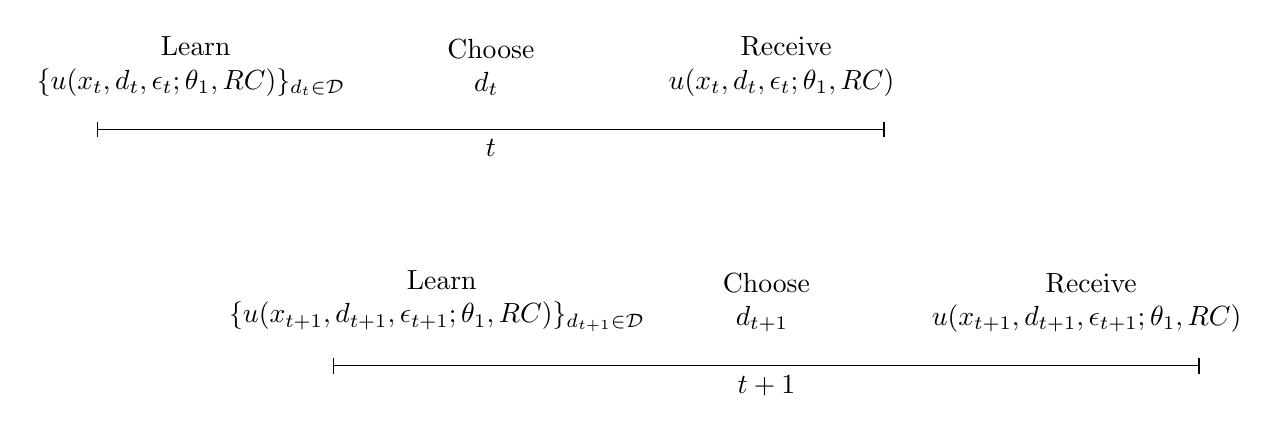
\begin{tikzpicture}
	\draw [|-|]
	(0,1) -- (10,1)
	node [above,align=center,very near start]
	{
		Learn\\
		$\{u(x_t, d_t, \epsilon_t; \theta_1, RC)\}_{d_t \in \mathcal{D}}$
		\vspace{2ex}
	}
	node [above,align=center,midway]
	{
		Choose\\
		$d_t$
		\vspace{2ex}
	}
	node [above,align=center,very near end]
	{
		Receive\\
		$u(x_t, d_t, \epsilon_t; \theta_1, RC)$
		\vspace{2ex}
	}
	node [below, align=center, midway]
	{$t$};
	\draw [|-|]
	(3,-2) -- (14,-2)
	node [above,align=center,very near start]
	{
		Learn\\
		$\{u(x_{t+1}, d_{t+1}, \epsilon_{t+1}; \theta_1, RC)\}_{d_{t+1} \in \mathcal{D}}$
		\vspace{2ex}
	}
	node [above,align=center,midway]
	{
		Choose\\
		$d_{t+1}$
		\vspace{2ex}
	}
	node [above,align=center,very near end]
	{
		Receive\\
		$u(x_{t+1}, d_{t+1}, \epsilon_{t+1}; \theta_1, RC)$
		\vspace{2ex}
	}
	node [below, align=center, midway]
	{$t+1$};

	\end{tikzpicture}
\end{figure}
\vspace{2.5ex}

The transition of the state vector ($x^i_t$, $\epsilon^i_t$) is assumed to follow a Markov process, i.e. the current state only depends on the previous one and hence the utility maximization problem is time-invariant. This means that the problem faced by Zurcher is the same for a given state $(x^i_t$, $\epsilon^i_t)$ irrespective of the time $t$ in which he has to make his choice. Dropping the bus index $i$ for convenience, the optimization problem of the agent gives rise to the following value function for a single bus:

\begin{equation}
V(x_t, \epsilon_t) = \max_{\{d_t, d_{t+1}, ... \}} \E \left[\sum_{\tau=t}^{\infty} \beta^{\tau - t} u(x_\tau, d_\tau, \epsilon_\tau; \theta_1, RC)\right]
\end{equation}

Solving this model leads to an optimal policy rule $\pi^* = (d^{\pi^*}_t(x_t, \epsilon_t))^\infty_t$.

\subsection{The Model Solving}

The solution to the above model can be characterized by the Bellman equation (\cite{Bellman.1954}) below:

\begin{equation}
	\begin{split}
		V(x, \epsilon) = &\max_{d} \{v(x, d; \theta_1, RC) + \epsilon(d) \\[+3mm]
		&+ \beta \int_{x'} \int_{\epsilon'} V(x', \epsilon') p(x', \epsilon'| x, \epsilon, d, \theta_2, \theta_3) dx' d\epsilon'\}
	\end{split}
\end{equation}

with $(x, \epsilon)$ being the current period and $(x', \epsilon')$ the next period state. \paragraph{}

\cite{Rust.1987} simplifies the above problem now by assuming \textit{conditional independence} on the transition probabilities of the state vector $p(.)$:

\begin{equation}
	p(x', \epsilon'| x, \epsilon, d, \theta_2, \theta_3) = p_2(\epsilon'|x';\theta_2)p_3(x'|x, d; \theta_3)
\end{equation}

with further assuming that $\epsilon(d)$ is following a bivariate i.i.d. extreme value distribution with $\theta_2$ being Euler's constant. \paragraph{}

After discretizing the possible, continuous values of the state variable $x$, Rust derives from the original Bellman equation above the following contraction mapping needed to solve the economic model:

\begin{equation}
	\label{eq9}
	\begin{split}
		EV(\hat x_k, d) = &\sum_{j=0}^{J} log \left\{ \sum_{d'\in\{0, 1\}}  exp[v(x', d'; \theta_1, RC) + \beta EV(x', d')]\right\} \\[+3mm]
		&\times p_3(x'|\hat x_k, d; \theta_3).
	\end{split}
\end{equation}

with

\[p_3(x'|\hat x_k, d; \theta_3) = \left\{
\begin{array}{lr}
	Pr\{x'=\hat x_{k+j}|\theta_3\}  & \mbox{if } d = 0 \\
	Pr\{x'=\hat x_{1+j}|\theta_3\} & \mbox{if } d = 1
\end{array}
\right.
\]

for $j=0, 1, ..., J$ indicating how many grid points the mileage state climbs up in the next period. \paragraph{}

In the above equation, $EV(.)$ denotes the unique fixed point to a contraction mapping $T_f(EV, \theta)$ on the full state space $\Gamma_f = \{(\hat x_k, d)|\hat x_k \in \mathbf{\hat x}, d \in \mathcal{D}\}$. Here, $\hat x_k$ represents the grid point $k$ of the state variable $x$ while $\hat x_1 = 0$. The number of possible $\hat x_k$ depends on the choice of the grid size $K$ set by the researcher. The set of possible grid points then is denoted as $\mathbf{\hat x} = \{\hat x_1, ..., \hat x_K\}$. All the variables $v$ depict current period variables while variables $v'$ display the possible value in the next period. The conditional probability function $p_3(.)$ indicates how likely it is that a bus moves up a specific amount of grid points in the next period depending on the structural parameter $\theta_3$ as well as the choice $d$. Imagine now we decide to set the grid size to $K=90$ as done in \cite{Rust.1987}, then we generally have to find the fixed point above which yields the solution $EV_f = (EV(\hat x_1, 0), ..., EV(\hat x_{90}, 0), EV(\hat x_1, 1), ..., EV(\hat x_{90}, 1))$. This simplifies, though, as all the expected values from $EV(\hat x_1, 1), ..., EV(\hat x_{90}, 1)$ are actually equivalent to $EV(\hat x_1, 0)$ due to the regenerative nature of the decision problem. This means that in our scenario we just have to solve the vector $(EV(\hat x_1, 0)\; ...\; EV(\hat x_K, 0))^T$ which I denote as $EV_r$ and we have the whole vector $EV_f$ at hand. In our example the vector $EV_r$ has a dimension of $90$. This observation will later be important for the difference between NFXP and MPEC. \cite{Su.Judd.2012}, hence, denote the dimension-reduced contraction mapping shorthand as:

\begin{equation}
EV_r = T_r(EV_r, \theta)
\end{equation}

with $T_r(.)$ being a contraction mapping on the reduced state space $\Gamma_r = \{(\hat x_k, d=0)|\hat x_k \in \mathbf{\hat x}\}$.

The unique fixed point can now be used to derive conditional choice probabilities of the agent:

\begin{equation}
	\label{eq11}
	P(d|\hat x; \theta) = \frac{exp[v(\hat x, d; \theta_1, RC) + \beta EV(\hat x, d)]}{\sum_{d' \in \{0, 1\}} exp[v(\hat x, d'; \theta_1, RC) + \beta EV(\hat x, d')]}.
\end{equation}

The above equation describes the probability that the agent chooses $d$ given that the observed mileage state is at a certain grid point $\hat x$. This derivation depends on both the cost parameters ($\theta_1$, $RC$) directly and indirectly through $EV(.)$ as well as on the transition parameter $\theta_3$. These conditional choice probabilities together with the transition probabilities $p_3(.)$ become relevant in the next section when calibrating the model using maximum likelihood.


\subsection{Calibration}

In order to calibrate the parameter vector $\theta =(\theta_1, \theta_3, RC)$ using either NFXP or MPEC, let us assume that we observe some data set $X = (X^i)^M_{i=1 }$ with $X^i = (x^i_t, d^i_t)^T_{t=1}$ for a single bus $i = 1, ..., M$. The data therefore consists of the engine replacement decision per bus and period as well as the cumulative mileage since the last engine replacement. The cumulative mileage $x^i_t$ is assumed to already be discretized which means that it takes values on the grid $\mathbf{\hat x} = \{\hat x_1, ..., \hat x_K\}$. The log likelihood of observing the data $X$ now becomes:

\begin{equation}
	L(\theta) = \sum_{i=1}^{M} \sum_{t=2}^{T} log[P(d^i_t|x^i_t; \theta)] + \sum_{i=1}^{M} \sum_{t=2}^{T} log[p_3(x^i_t|x^i_{t-1}, d^i_{t-1}; \theta_3)].
\end{equation}

To fulfill the aim of finding the optimal parameter vector $\theta$ one now has to solve the problem of maximizing the above log likelihood:

\begin{equation}
	\max_{\theta} L(\theta).
\end{equation}

The path taken by the NFXP is now to hand this unconstrained optimization problem to an optimization algorithm such as the Berndt-Hall-Hall-Hausman (BHHH) algorithm based on \cite{Berndt.1974}. The algorithm comes up with a guess for the optimal parameter $\hat \theta$ for which in a subroutine the expected values in equation \ref{eq9} are calculated. The expected value function is in turn needed to obtain the conditional choice probabilities in equation \ref{eq11} which are then taken to evaluate the log likelihood $L(\theta)$. Based on this evaluation, the optimization algorithm comes up with a new guess for $\hat \theta$ and the above procedure is repeated until a certain convergence criteria of the algorithm is met. This procedure is again shown in pseudocode in Algorithm \ref{alg3} on the next page.

At every structural guess of the optimization algorithm the fixed point $EV(.)$ is calculated precisely as it is needed to evaluate the log likelihood $L(\theta)$. This is deemed inefficient by \citeauthor{Su.Judd.2012} which gives rise to the augmented log likelihood mentioned before for which they insert the conditional choice probabilities $P(d^i_t|x^i_t; \theta)$ into $L(\theta)$ making the log likelihood explicitly depend on $EV(.)$. This results in the following log likelihood:

\vspace{2ex}
\begin{algorithm}[!h]
	\caption{Nested Fixed Point Algorithm for the Rust Model}
	\label{alg3}
	\SetAlgoLined
	\KwIn{$\hat\theta_n$, $n=0$, $X$\;}
	\While{$f(|| (\hat\theta_{n+1}, \hat{EV}_{n+1}) - (\hat\theta_{n}, \hat{EV}_{n}) ||) \geq$ stopping tolerance}{
		\vspace{2ex}
		Solve fixed point
		\begin{equation*}
		EV(\hat x_k, d) = \sum_{j=0}^{J} log \left\{ \sum_{d'\in\{0, 1\}}  exp[v(x', d'; \hat \theta_{n, 1}, \hat{RC_n}) + \beta EV(x', d')]\right\} \times p_3(x'|\hat x_k, d; \hat \theta_{n, 3});
		\end{equation*}

		Given the solution to $EV(.)$ calculate
		\begin{flalign*}
		P(d|\hat x; \hat \theta_n) = \frac{exp[v(\hat x, d; \hat \theta_{n, 1}, \hat{RC_n}) + \beta EV(\hat x, d)]}{\sum_{d' \in \{0, 1\}} exp[v(\hat x, d'; \hat \theta_{n, 1}, \hat{RC_n})) + \beta EV(\hat x, d')]};
		\end{flalign*}

		Evaluate the log likelihood
		\begin{flalign*}
		L(\hat \theta_n) = \sum_{i=1}^{M} \sum_{t=2}^{T} log[P(d^i_t|x^i_t; \hat \theta_n)] + \sum_{i=1}^{M} \sum_{t=2}^{T} log[p_3(x^i_t|x^i_{t-1}, d^i_{t-1}; \hat \theta_{n, 3})];
		\end{flalign*}

		Based on that fix a new guess $\hat\theta_{n+1}$\;
	}
\end{algorithm}
\vspace{2ex}

\begin{equation}
\begin{split}
\mathcal{L}(\theta, EV) = &\sum_{i=1}^{M} \sum_{t=2}^{T} log \left[\frac{exp[v(x^i_t, d^i_t, \theta) + \beta EV(x^i_t, d^i_t)]}{\sum_{d' \in \{0, 1\}}exp[v(x^i_t, d', \theta) + \beta EV(x^i_t, d')]}\right] \\[+3mm]
&+ \sum_{i=1}^{M} \sum_{t=2}^{T} log[p_3(x^i_t|x^i_{t-1}, d^i_{t-1}; \theta_3)].
\end{split}
\end{equation}

In this function nothing guarantees that $\theta$ and $EV$ are actually consistent. This is healed by imposing the fixed point equation \ref{eq9} as constraints to the augmented likelihood function. The MPEC formulation of the calibration problem therefore looks like the following.

\begin{equation}
\begin{aligned}
& \max_{(\theta, EV)} \mathcal{L}(\theta, EV) \\
& \text{subject to } EV = T(EV, \theta).
\end{aligned}
\label{eq2}
\end{equation}

For the MPEC formulation the problem is given to an optimization algorithm that can handle nonlinear equality constraints such as the already mentioned KNITRO or IPOPT. This algorithm then fixes a guess of $(\theta, EV)$ that satisfies the nonlinear constraints, i.e. that is consistent with the underlying economic model and for which the augmented log likelihood is evaluated. Based on this evaluation, the optimizer determines a new guess and the procedure starts over. Again this is done until a specific convergence criteria is met. This procedure is illustrated in Algorithm \ref{alg4} on the next page.


\vspace{2ex}
\begin{algorithm}[!h]
	\caption{MPEC Algorithm for the Rust Model}
	\label{alg4}
	\SetAlgoLined
	\KwIn{$\hat\theta_n$, $\hat{EV_n}$, $n=0$, $X$\;}
	\While{$f(|| \hat\theta_{n+1} - \hat\theta_{n} ||) \geq$ stopping tolerance}{
		\vspace{2ex}
		Evaluate the augmented log likelihood

		\begin{equation*}
		\begin{split}
		\mathcal{L}(\hat\theta_n, \hat{EV_n}) = &\sum_{i=1}^{M} \sum_{t=2}^{T} log \left[\frac{exp[v(x^i_t, d^i_t, \hat\theta_n) + \beta \hat{EV_n}(x^i_t, d^i_t)]}{\sum_{d' \in \{0, 1\}}exp[v(x^i_t, d', \hat\theta_n) + \beta \hat{EV_n}(x^i_t, d')]}\right] \\[+3mm]
		&+ \sum_{i=1}^{M} \sum_{t=2}^{T} log[p_3(x^i_t|x^i_{t-1}, d^i_{t-1}; \hat\theta_{n, 3})]
		\end{split}
		\end{equation*}

		Based on that fix a new guess $(\hat\theta_{n+1}, \hat{EV}_{n+1})$\;
	}
\end{algorithm}
\vspace{2ex}

Having established both NFXP and MPEC for the Rust model, let us now turn to some particularities of the model that might be important for the performance of the two algorithms. First of all, \cite{Rust.1987} and \cite{Su.Judd.2012} show that both the likelihood for the NFXP and the MPEC are smooth for the Rust model and their first and second order derivatives exist. In the case of the NFXP this means that Newton's method can be used for the maximization problem. It also helps modern solvers such as KNITRO and IPOPT which are developed for smooth optimization problems (compare \cite{Byrd.Nocedal.Waltz.2006} and \cite{Waechter2009}). Another special feature is that solving the model involves finding a fixed point. In the case of the NFXP it is time consuming to find as it involves contraction iterations. This caused Rust to employ a polyalgorithm to find the fixed point using contraction steps at the beginning and switching to Newton-Kantorovich (N-K) steps as soon as a guess is already close to the unique fixed point. This practically speeds up the convergence when searching for the fixed point as contraction iterations solely have a linear convergence rate while N-K iterations converge at a quadratic rate when being close to the fixed point (see \cite{Rust.1987, Rust.2000}). As already noted before, MPEC on the other hand does not solve the fixed point but instead evaluates it once at every structural parameter guess without high precision until the last iteration of the optimization procedure. Another factor explained in the general part on MPEC is the high dimensionality of its problem formulation. Going back to our example when the grid size is set to $90$, the MPEC formulation yields a problem consisting of $90$ nonlinear constraints and $90 + |\theta|$ parameters to estimate. The NFXP has considerably less dimensions as only $|\theta|$ parameters have to be estimated and no constraints have to be considered by the optimizer. \cite{Su.Judd.2012} uncover the trade off of dimensionality and fixed point calculation to be the major one between MPEC and NFXP in the Rust model application. Following this line of arguments it is not obviously clear how the chosen grid size affects this trade off as the grid size increases the dimensions of the MPEC problem while also making the fixed point calculation in the NFXP more computationally expensive.

\subsection{General Setup and Replication} \label{generalsetup}

For the remainder of this thesis I rely on the open-source Python package ruspy which was initially created by \cite{Blesch.2019}. In this package, he implements Rust's Nested Fixed Point Algorithm based on \cite{Rust.2000}. I adjusted the code for the NFXP to be capacable of replicating \cite{Iskhakov.2016}. Further I entirely added the MPEC implementation for the Rust model based on the explanations in the aforementioned paper as well as in \cite{Su.Judd.2012} \footnote{Please refer to Pull Requests \href{https://github.com/OpenSourceEconomics/ruspy/pull/42}{\#42} and \href{https://github.com/OpenSourceEconomics/ruspy/pull/46}{\#46} to view my contributions to the ruspy package.}\textsuperscript{,}\footnote{The previous version of ruspy only implemented Quasi-Newton Methods based on the scipy library (see \cite{scipy.2020}). The library does not offer the BHHH algorithm used for the NFXP in \cite{Iskhakov.2016}. I added the BHHH to the estimagic library (see \cite{Gabler.2019}) in the Pull Request \href{https://github.com/OpenSourceEconomics/estimagic/pull/161}{\#161} in order to use it for ruspy.}. To grasp why \citeauthor{Iskhakov.2016} follow up on \citeauthor{Su.Judd.2012} with a revised setup of MPEC and NFXP for the Rust model, let us go back to the latter paper. After having set up the theoretical implications of MPEC as outlined in the above sections, \citeauthor{Su.Judd.2012} conclude with a practical implementation of both approaches in a Monte Carlo simulation of the Rust model. Their finding is that MPEC is not only easier to code up but also significantly faster than the NFXP especially when the discount factor is close to one. Further MPEC has a higher convergence rate. \citeauthor{Iskhakov.2016} intervene now arguing that the NFXP implementation relied on by \citeauthor{Su.Judd.2012} is inferior to the one suggested by \cite{Rust.2000}. This is mainly due to the fact that they do not use the BHHH for the likelihood optimization and further do not employ the polyalgorithm of contraction and Newton-Kantorovich iterations but solely contraction iterations for the fixed point calculation. \citeauthor{Iskhakov.2016} further add an improvement to the MPEC implementation which I also accounted for in my code. They recenter the expected value function to make it more numerically stable which improves the implementation especially when the discount factor $\beta$ is very close to one. In a last step, the authors draw on the same data generating process in a Monte Carlo simulation as was done by \citeauthor{Su.Judd.2012} and show that with their setup MPEC and NFXP are similarly fast and that both have a very high convergence rate. In my own implementation I stay as closely as possible to the setup employed by \citeauthor{Iskhakov.2016} given some notable differences that I explain in section \ref{appendixA} in the appendix.

For the simulation studies in the rest of this thesis, unless otherwise stated, I hence follow the data generating process of \cite{Iskhakov.2016} which looks like the following. There are 120 time periods, i.e. $T=120$ and 50 buses, i.e. $M=50$ that are simulated. The cost function $c(x; \theta_1)$ is assumed to be linear with a scale parameter of $0.001$, i.e. $c(x; \theta_{11}) = 0.001 \times \theta_{11} x$. The true parameters are the following:

\begin{equation*}
	\begin{split}
		& RC = 11.7257 \\
		& \theta_{11} = 2.4569 \\
		& \theta_3 = \begin{pmatrix}
		0.0937 & 0.4475 & 0.4459 & 0.0127 & 0.0002
		\end{pmatrix}
	\end{split}
\end{equation*}

with $\theta_3$ being the Markovian probability that the state of a bus in a given period of time moves up zero, one, two, three or four grid points concerning the mileage state $x$, respectively. This refers back to equation \ref{eq9}.

As the Rust model does not allow to estimate the discount factor $\beta$, it has to be predetermined as well. The true parameter for $\beta$ is consequently varied in the following setups as it affects how easily the fixed point for $EV(.)$ can be found.

\begin{equation*}
	\beta \in \{0.975, 0.985, 0.995, 0.999, 0.9995, 0.9999\}
\end{equation*}

For each possible $\beta$, 250 data sets following the Rust model with the above parameters are simulated. In order to check for the robustness of the two approaches to different starting values, those are varied as well and each data set is estimated five times using the following different starting parameter guesses:

\begin{equation*}
	(RC^0, \theta^0_{11}) \in \{(4,1), (5, 2), (6, 3), (7, 4), (8, 5)\}.
\end{equation*}

The continuous mileage state is discretized into a grid of 175 points, meaning that the unique fixed point of the expected values $EV$ is 175-dimensional vector. In the case of MPEC, also starting values for this vector have to be passed in which are always set to:

\begin{equation*}
	\begin{pmatrix} EV_1 \\ \vdots \\ EV_{175} \end{pmatrix} = \begin{pmatrix} 0 \\ \vdots \\ 0 \end{pmatrix}.
\end{equation*}

For MPEC the algorithm IPOPT is utilized while \citeauthor{Iskhakov.2016} as well as \citeauthor{Su.Judd.2012} take KNITRO. The latter is a commercial optimizer which cannot be used for a generally open-source package such as ruspy which is why in that package we offer only NLOPT and IPOPT. IPOPT is used in its default settings with a relative stopping tolerance of $10^{-6}$. I pass in upper bounds of $50$ for the $EV$ vector and lower bounds of zero for $RC$ and $\theta_{11}$ to the optimizer. Further the first order analytical derivative of the Langrangian of the constrained optimization problem is supplied.\paragraph{}

\begin{table}[H]
	\centering
	\caption{Replication of Iskhakov et al. (2016)}
	\label{table1}
	\begin{tabular}{l c c c c c c}
		\toprule\midrule
		$\beta$ & Converged  & CPU Time & \# of Major & \# of Func. & \# of Bellm. & \# of N.K.   \\
		& (Out of 1250) & (in Sec.) & Iter. & Eval. & Iter. & Iter. \\
		\midrule
		\multicolumn{7}{c}{\textbf{MPEC-IPOPT}} \\
		0.975 & 1250 & 1.151 & 19.6 & 25.9 \\
		0.985 & 1250 & 1.187 & 19.9 & 28.4 \\
		0.995 & 1250 & 1.352 & 22.2 & 35.1 \\
		0.999 & 1249 & 1.613 & 25.3 & 41.5 \\
		0.9995 & 1248 & 1.754 & 26.1 & 43.6 \\
		0.9999 & 1250 & 1.861 & 28.1 & 49.3 \\
		\multicolumn{7}{c}{\textbf{NFXP}} \\
		0.975 & 1250 & 1.286 & 11.8 & 14.1 & 301.7 & 104.4 \\
		0.985 & 1250 & 1.306 & 11.4 & 13.6 & 291.2 & 105.6 \\
		0.995 & 1250 & 1.185 & 10.6 & 12.7 & 272.9 & 97.7 \\
		0.999 & 1250  & 1.556 & 10.9 & 12.9 & 278.0 & 138.4 \\
		0.9995 & 1250 & 2.626 & 10.9 & 12.9 & 277.6 & 250.7 \\
		0.9999 & 1250 & 2.778 & 10.9 & 12.9 & 276.6 & 270.0 \\
		\bottomrule
	\end{tabular}
\end{table}

As previously stated, the NFXP is implemented as a polyalgorithm for the fixed point calculation and the BHHH for likelihood optimization is applied. For the BHHH I choose a relative stopping tolerance of $10^{-8}$ as well as $10^{-5}$ as an absolute stopping tolerance. The switching tolerance from contraction to N-K steps is set to $10^{-2}$ while the stopping tolerance for the fixed point calculation is fixed at $10^{-13}$. In the case of NFXP as well the analytical first order derivative of the likelihood function is provided to the optimizer. Now, I use this setup to estimate the structural parameters of the original data sets that have been created by \citeauthor{Iskhakov.2016} in their Monte Carlo simulation with the above outlined data generating process. The results are presented in Table \ref{table1}.

As already mentioned, both MPEC and NFXP are implemented differently and run on a different computer than in the original paper making the absolute comparison of numbers fruitless. What can be seen, though, is that also when using a similar implementation to them with another programming language (they use matlab and AMPL) in the general structure similar results can be achieved. The convergence rates are very high (even higher for my implementation of MPEC than for the one of \citeauthor{Iskhakov.2016}). The CPU time is on a similar level for both MPEC and NFXP given a specific discount factor. We can observe that with rising $\beta$ the fixed point calculation becomes more complex indicated by the rising number of N-K steps needed to solve it. The implementation of \cite{Iskhakov.2016} is more stable in this regard which is likely explained by the fact that they also allow for back switching from N-K to contraction iterations. For MPEC the increased difficulty of solving for the fixed point translates into more iterations and function evaluations needed. As opposed to the original paper where also the analytical Hessian as well as its sparsity pattern and that of the Jacobian of the Lagrangian are provided, my less complex implementation performs remarkably well.

This section constitutes the starting point of a part of my remaining discussions in which I test how reactive NFXP and MPEC are to certain criteria of the model and how this translates into qualitative differences using another variable of comparison than \cite{Su.Judd.2012} as well as \cite{Iskhakov.2016}. This other dimension is the uncertainty around a quantity of interest which I will introduce in the upcoming section.


\section{Uncertainty Quantification} \label{uq}
\thispagestyle{plain} % surpress header on first page

Most sciences work at least to a certain degree quantitatively and by doing so they often rely on theoretical models that in many cases approximate the underlying true mechanisms that drive a certain process or phenomenon. In many cases the quantitative model outcome of interest is the result of a transformation of model inputs through a complex mathematical system. Across disciplines, from a model perspective many inputs and initial states as well as their development are not deterministic but are uncertain. The model inputs are often informed by theory, previous quantitative studies as well as experiments or need to be calibrated using limited data but cannot be treated as known. It is now often argued that the inherently uncertain parameters propagate their error through the model which yields an uncertain model outcome. In order to make informed decisions based on the model outcome, this uncertainty should be quantified and communicated. This constitutes one main motivation why the applied mathematics field of Uncertainty Quantification (UQ) developed and still is an active field of research. Many of its advancements come from the engineering and physical sciences in which negligence of uncertainty in the outcomes can lead to attributable and severe consequences. In climatology, the predicted path of a hurricane is reported with uncertainties which are due to the dynamical, complex weather conditions that can only be approximated. These uncertainties inform countries about whether they might be hit while giving them valuable time to prepare. An example from engineering involves the safety of a nuclear power plant which in turn is affected by factors such as the weather and its environment in general. This also includes seismological activity which was causing the catastrophe in Fukushima back in 2011. Uncertainty Quantification tries to incorporate those risks in the modeling process and make them explicit (compare \cite{Sullivan.2015} and \cite{Smith.2013}).

Taking a step back from those very precise motivations for UQ, \cite{Smith.2019} make a simple mathematical point suggesting that it is worth to investigate uncertainty. Their motivation rests on the butterfly effect (see \cite{Lorenz.1963}) which demonstrates that already a slight perturbation in initial conditions can result in an unforeseeable change in the outcome of a complex dynamical system over time. Going back to our initial observation that models often are complex mathematical systems, this provokes the thought that also in this case small changes in inputs might have a strong impact on model predictions. But how does that matter in Economics? And how do we quantify this uncertainty? An answer to the first question and a motivation for UQ can be found in a recent study by \cite{Cai.2019}. They estimate "the social cost of carbon (SCC), defined as the marginal economic loss caused by an extra metric ton of atmospheric carbon" \footnote{ Compare page 3 in \cite{Cai.2019}.} based on the Dynamic Integrated Climate–Economy” (DICE) model (\cite{Nordhaus.1992, Nordhaus.2008}). They add uncertainty regarding the economic development as well as the change in climate conditions to this framework by assuming possible ranges of those factors and propagate them through their model. The result is quite astonishing as for the year 2005 the SCC varies between 59 to 99 Dollars per ton of carbon for a realistic range of projections in economic and climatic outlook. This range of uncertainty in the model outcome is quite large but clearly sends a more informative message to policy makers.

While it is well understood in Economics that there is uncertainty affecting model outcomes and hence policy recommendations as well as that its communication is crucial, it is rarely the case that a full, coherent evaluation of uncertainties is performed that goes beyond robustness checks (see \cite{Manski.2019} and \cite{Scheidegger.2019}). This is where the already existent UQ framework can come in and answer the second question from before, how to quantify uncertainty and determine which sources are contributing to it as recently done in \cite{Scheidegger.2019} and in \cite{Harenberg.2019}. In the following, I will introduce the cornerstones of this framework and apply some of its general ideas to the Rust model and the comparison of MPEC and the NFXP.

\subsection{The UQ Framework}

For the following description I mainly rely on \cite{Smith.2013} who outlines a comprehensive UQ framework with a focus on engineering and physics as well as on \cite{Oberkampf.2010} who deal with uncertainty in a more general scientific computing context.  The starting point for both is the observation that there are many potential sources of uncertainty that can affect the outcome of a computational model. First, there is model uncertainty which translates into the underlying mathematical framework of a model. In many cases the true underlying process that the mathematical model is supposed to capture is not perfectly understood which renders the mathematical representation imprecise. In the Rust Model we impose the behavioral assumption on Harold Zurcher that his decision process follows that of a maximization of his discounted life time utility over an infinite horizon. We do not know whether this is warranted and even if it was, on a lower level there is still uncertainty about how his underlying cost function exactly looks like for example. Quite obviously the choice of the specific mathematical representation affects the predictions the model will make after being calibrated. A second source are the parameter inputs themselves. As in Economics they usually are estimated from data, there always remains uncertainty around the specific parameter estimates. This parameter uncertainty translates into uncertainty of the model outcomes. Thirdly, in many applications the computational implementation of a mathematical model involves approximate numerical solutions to the whole model itself or at least parts of it. In our example, we rely on numerical optimization algorithms that introduce some error but also the discretization of the expected value function is solely an approximation of the true mathematical relation. A last factor is a potential measurement error in the model inputs. This could be for instance an imprecise measurement of the cumulative mileage state of some buses.

The authors argue now that the very nature of those uncertainties can be different. On the one hand, the uncertainty can be \textit{aleatoric} which means that it is stochastic and cannot be reduced by gaining additional economic or experimental knowledge. For those uncertainties there typically exists a probability distribution. On the other hand, there is \textit{epistemic} uncertainty which can generally be reduced. It includes for example the previously stated uncertainty of the correct cost function which might be solved by running an experiment. For this example, there clearly is no probability distribution describing the error but rather an interval of different possible uncertainties. Given that some of these uncertainties are uncovered in a specific model, the UQ framework prescribes the following two steps. However, before we dive into this, let us first refine the terms of model and model outcome. In the UQ framework, the computational model can be described like this:

\begin{equation}
	y = f(\theta)
	\label{compmodel}
\end{equation}

where $\theta$ are the model inputs or parameters and $y \in \mathbb{R}^Q$ the model output or the quantity of interest (QoI). \paragraph{}
The QoI can be any policy relevant vector or scalar that could be obtained from the underlying mathematical model. In \cite{Cai.2019} this is the social cost of carbon. In my thesis, this will be some counterfactual demand level for bus engines given a certain replacement cost. I will further go into detail about this in the next section. This computational model itself can already suffer from discrepancies to the true mathematical model due to model errors and numerical errors. Given that the model parameters have to be calibrated from data and hence suffer from uncertainty in the estimates, they are represented by a random vector $\Theta$ which has a certain probability distribution depending on the data at hand. Given the calibrated parameters, the uncertainty in the parameters affect the model outcome in the following way:

\begin{equation}
	Y = f(\Theta)
	\label{uncertaincompmodel}
\end{equation}

with $Y$ being the QoI that itself is a random vector or variable. \paragraph{}

The fact that measurement, numerical and model uncertainty might exist is implicitly included in the fact that the computational model $f(.)$ is not equivalent to the true mathematical model, i.e. the QoI $y$ and the parameter vector $\theta$ are already not deterministic but rather uncertain affected by the above mentioned errors.

Coming back to our two steps in the UQ framework, first, the uncertainties are accounted for in the model inputs and then propagated through the model. Second, this propagation is then accounted for in some uncertainty around the quantity of interest. In a sub field of UQ, \textit{sensitivity analysis}, this propagation technique is exploited to determine which parameters of the model contribute the most to the observed uncertainty in the QoI. This can be of great interest even beyond the argument of informed policy decisions as it can give valuable information to researchers that want to calibrate a certain economic model with actual data. It gives them an indication which parameters to focus on during the calibration procedure which in turn might reduce the uncertainty in the QoI. This analysis further conveys information about the mathematical model itself an how it could be refined to provoke a lower uncertainty around the QoI (see \cite{Scheidegger.2019},  \cite{Harenberg.2019} and \cite{Ghanem.2017}). In this literature, usually a host of combinations of different parametrizations are used to propagate through the model and calculate its QoI. This information from several runs is then used to systematically determine the influence of the uncertainty in certain parameters on the uncertainty in the QoI. With increasing complexity of the computational model, this becomes computationally infeasible as it would involve too many runs of the model. This is the reason why the literature developed so called surrogate models that approximate the true computational model while maintaining higher speed of convergence for a single run (compare also \cite{Saltelli.2008}). While this strand of literature focuses on parameter uncertainty, in the setting of economic models it also implicitly takes some other forms of uncertainty from the calibration procedure into account as the exact estimate of a parameter depends also on model and numerical specifications in the calibration procedure. In many cases, though, a potential model or numerical error will also affect the QoI directly and not solely through the parameter uncertainty as will be the case in what is about to follow.

First, though, in the following section I will introduce the mathematical and computational model for the QoI from which the remainder of my thesis will draw.

\subsection{The Quantity of Interest: The Demand Function}

\cite{Rust.1987} shortly describes a way to uncover an implied demand function of engine replacement from his model in combination with estimated parameters. Theoretically, for Harold Zurcher the random annual implied demand function takes the following form:

\begin{equation*}
	\tilde{d}(RC) = \sum_{t=1}^{12} \sum_{m=1}^{M} \tilde{d}^m_t
\end{equation*}

while $\tilde{d}^m_t$ is the replacement decision for a certain bus $m$ in a certain month $t$ derived from the process \{$d^m_t$, $x^m_t$\}. For convenience I will drop the index for the bus in the following. Its probability distribution is therefore the result of the process described by $P(d_t|x_t; \theta)p_3(x_t|x_{t-1}, d_{t-1}; \theta_3)$. For simplification \citeauthor{Rust.1987} actually derives the expected demand function $d(RC)=\E[\tilde{d}(RC)]$. Assuming that $\pi$ is the long-run stationary distribution of the process \{$d_t$, $x_t$\} and that the observed initial state \{$x_0$, $d_0$\} is in the long run equilibrium, $\pi$ can be described by the following functional equation:

\begin{equation}
	\label{eq18}
	\pi(x, d; \theta) = \int_{y} \int_{j} P(d|x; \theta)p_3(x|y, j; \theta_3) \pi(dy, dj; \theta).
\end{equation}

Further assuming that the processes of \{$d_t$, $x_t$\} are independent across buses the annual expected implied demand function boils down to:

\begin{equation}
	\label{eq19}
	d(RC) = 12 M \int_{0}^{\infty} \pi(dx, 1; \theta).
\end{equation}

Given some estimated parameters $\hat\theta$ from calibrating the Rust Model and parametrically varying $RC$ results in different estimates of $P(d_t|x_t; \theta)p_3(x_t|x_{t-1}, d_{t-1}; \theta_3)$ which in turn affects the probability distribution $\pi$ which changes the implied demand. In the representation above it is clearly assumed that both the mileage state $x$ and the replacement decision $d$ are continuous. The replacement decision is actually discrete, though, and the mileage state has to be discretized again which in the end results in a sum representation of equation \ref{eq18} that is taken to calculate the expected annual demand function.
\paragraph{}

A flexible calculation of the above demand function depending on some parameter vector $\theta$ has been implemented by me in the ruspy package which I will rely on in the following. I will now showcase the UQ framework for uncertainty propagation by using the resulting empirical distribution function of the parameter vector $\hat\theta$ from the Monte Carlo simulation in \ref{generalsetup}, propagate it through the model (the calculation of the demand function) and obtain the distribution of a QoI (a certain demand level for a given $RC$) and consequently the uncertainty in its estimate.

\subsection{Uncertainty Propagation of the Simulation in Iskhakov et al. (2016)}

For this section I draw on the results of the Monte Carlo simulation for the discount factor $\beta=0.975$ from section \ref{generalsetup}. As the results for MPEC and NFXP are virtually the same and they do not vary across different starting values, I rely on the MPEC results for the starting values $(RC^0, \theta^0_{11}) = (4,1)$.

\begin{figure}[!t]
	\caption{Joint Distribution of $\hat{RC}$ and $\hat\theta_{11}$}
	\centering
	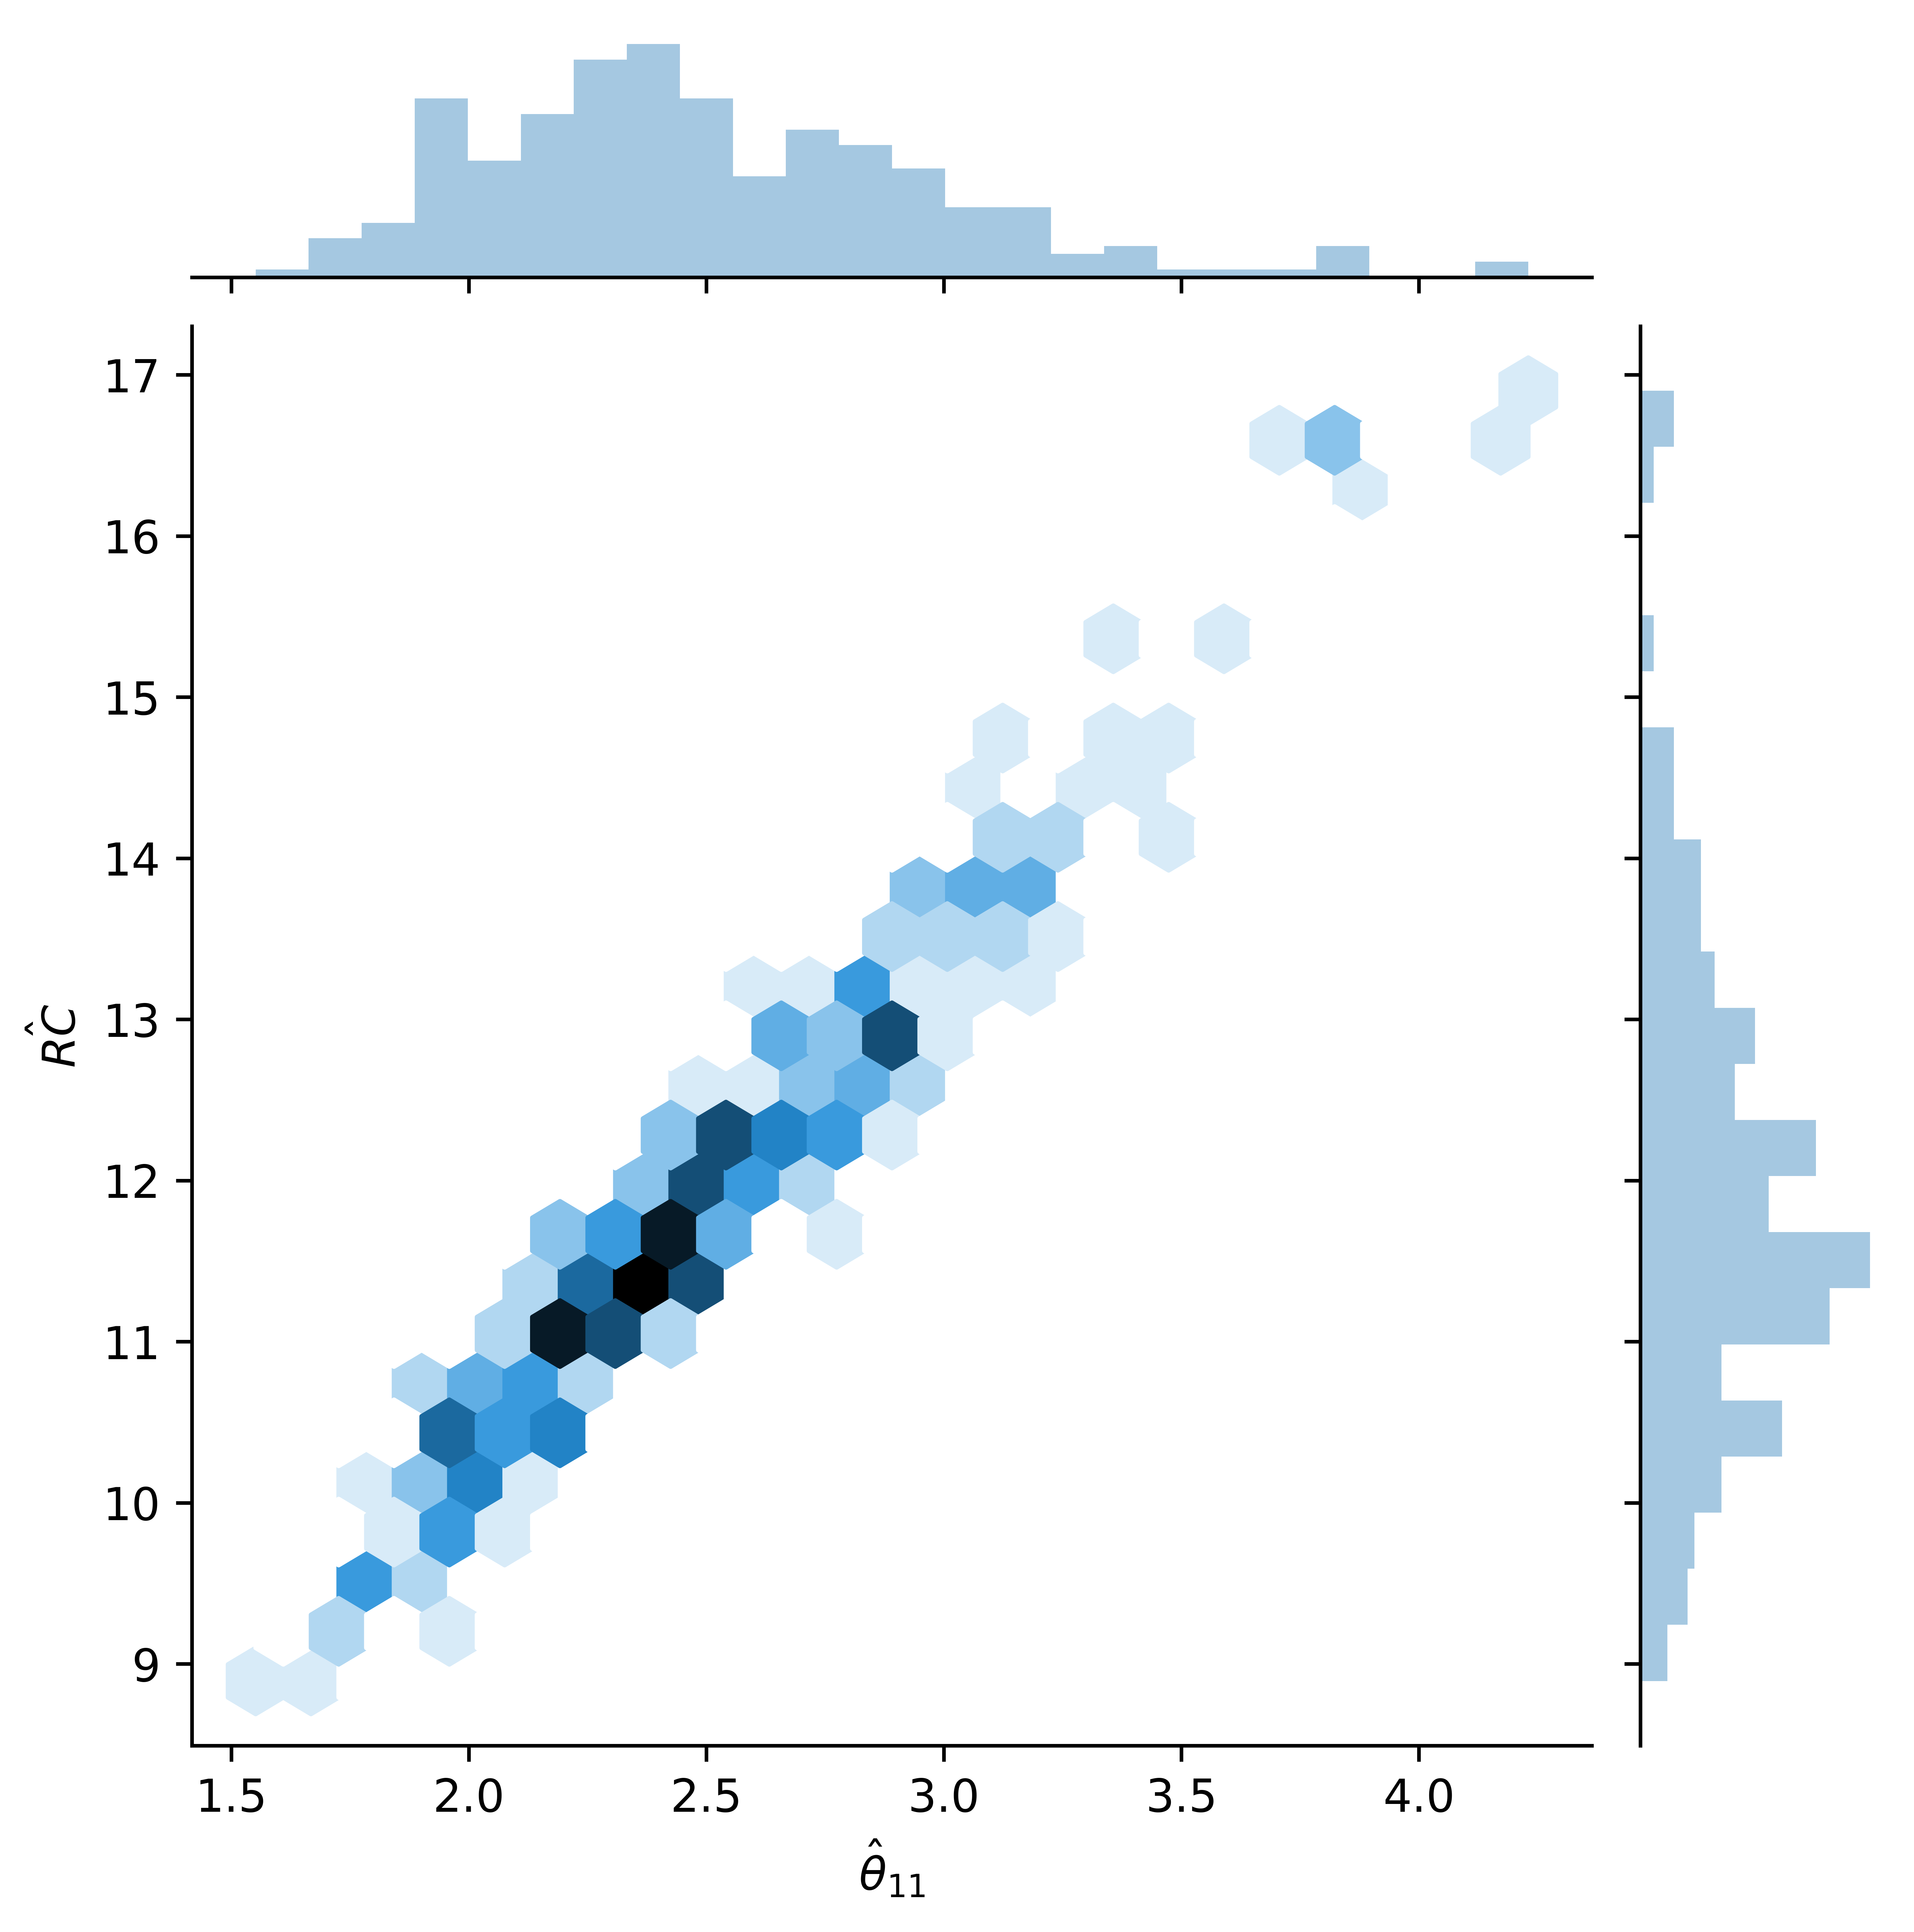
\includegraphics[scale=0.8]{../figures/figure_2.png}
	\label{figure2}
\end{figure}

Hence, in total I have 250 parameter estimates for 250 different data sets that were, as \cite{Su.Judd.2012} point out, created by a parametric bootstrap procedure. This allows me to identify summary statistics for both the parameters as well as the QoI. As we keep both the model assumptions and numerical approximations constant across the runs, we solely have a look at the effect of uncertainty in the parameters from the calibration process on the QoI. In the context of \textit{sensitivity analysis} which is targeting the influence of parameter uncertainty it is important to first determine whether the uncertainty in parameters is actually independent across them or whether there is some interdependence as it determines which techniques can actually give reliable results (\cite{Saltelli.2008}). The correlation between all parameters is reported in Table \ref{table2} in the appendix B. Here, I visualize the joint distribution of the cost parameter estimates in Figure \ref{figure2} which shows that there is a strong interdependence between them. Consequently, an approach to sensitivity analysis in which only one parameter at a time is varied to determine its contribution to the uncertainty in the QoI would lead to wrong results. In the above Figure \ref{figure2} we can further observe that the empirical distribution of our estimates is centered around the true values of the cost parameters and that the actual overestimation of them (compare to the appendix \ref{appendixC}) seems to be driven by some outliers that yield estimates being way too large.

\begin{figure}[!t]
	\caption{Distribution of the QoI}
	\vspace*{-4mm}
	\centering
	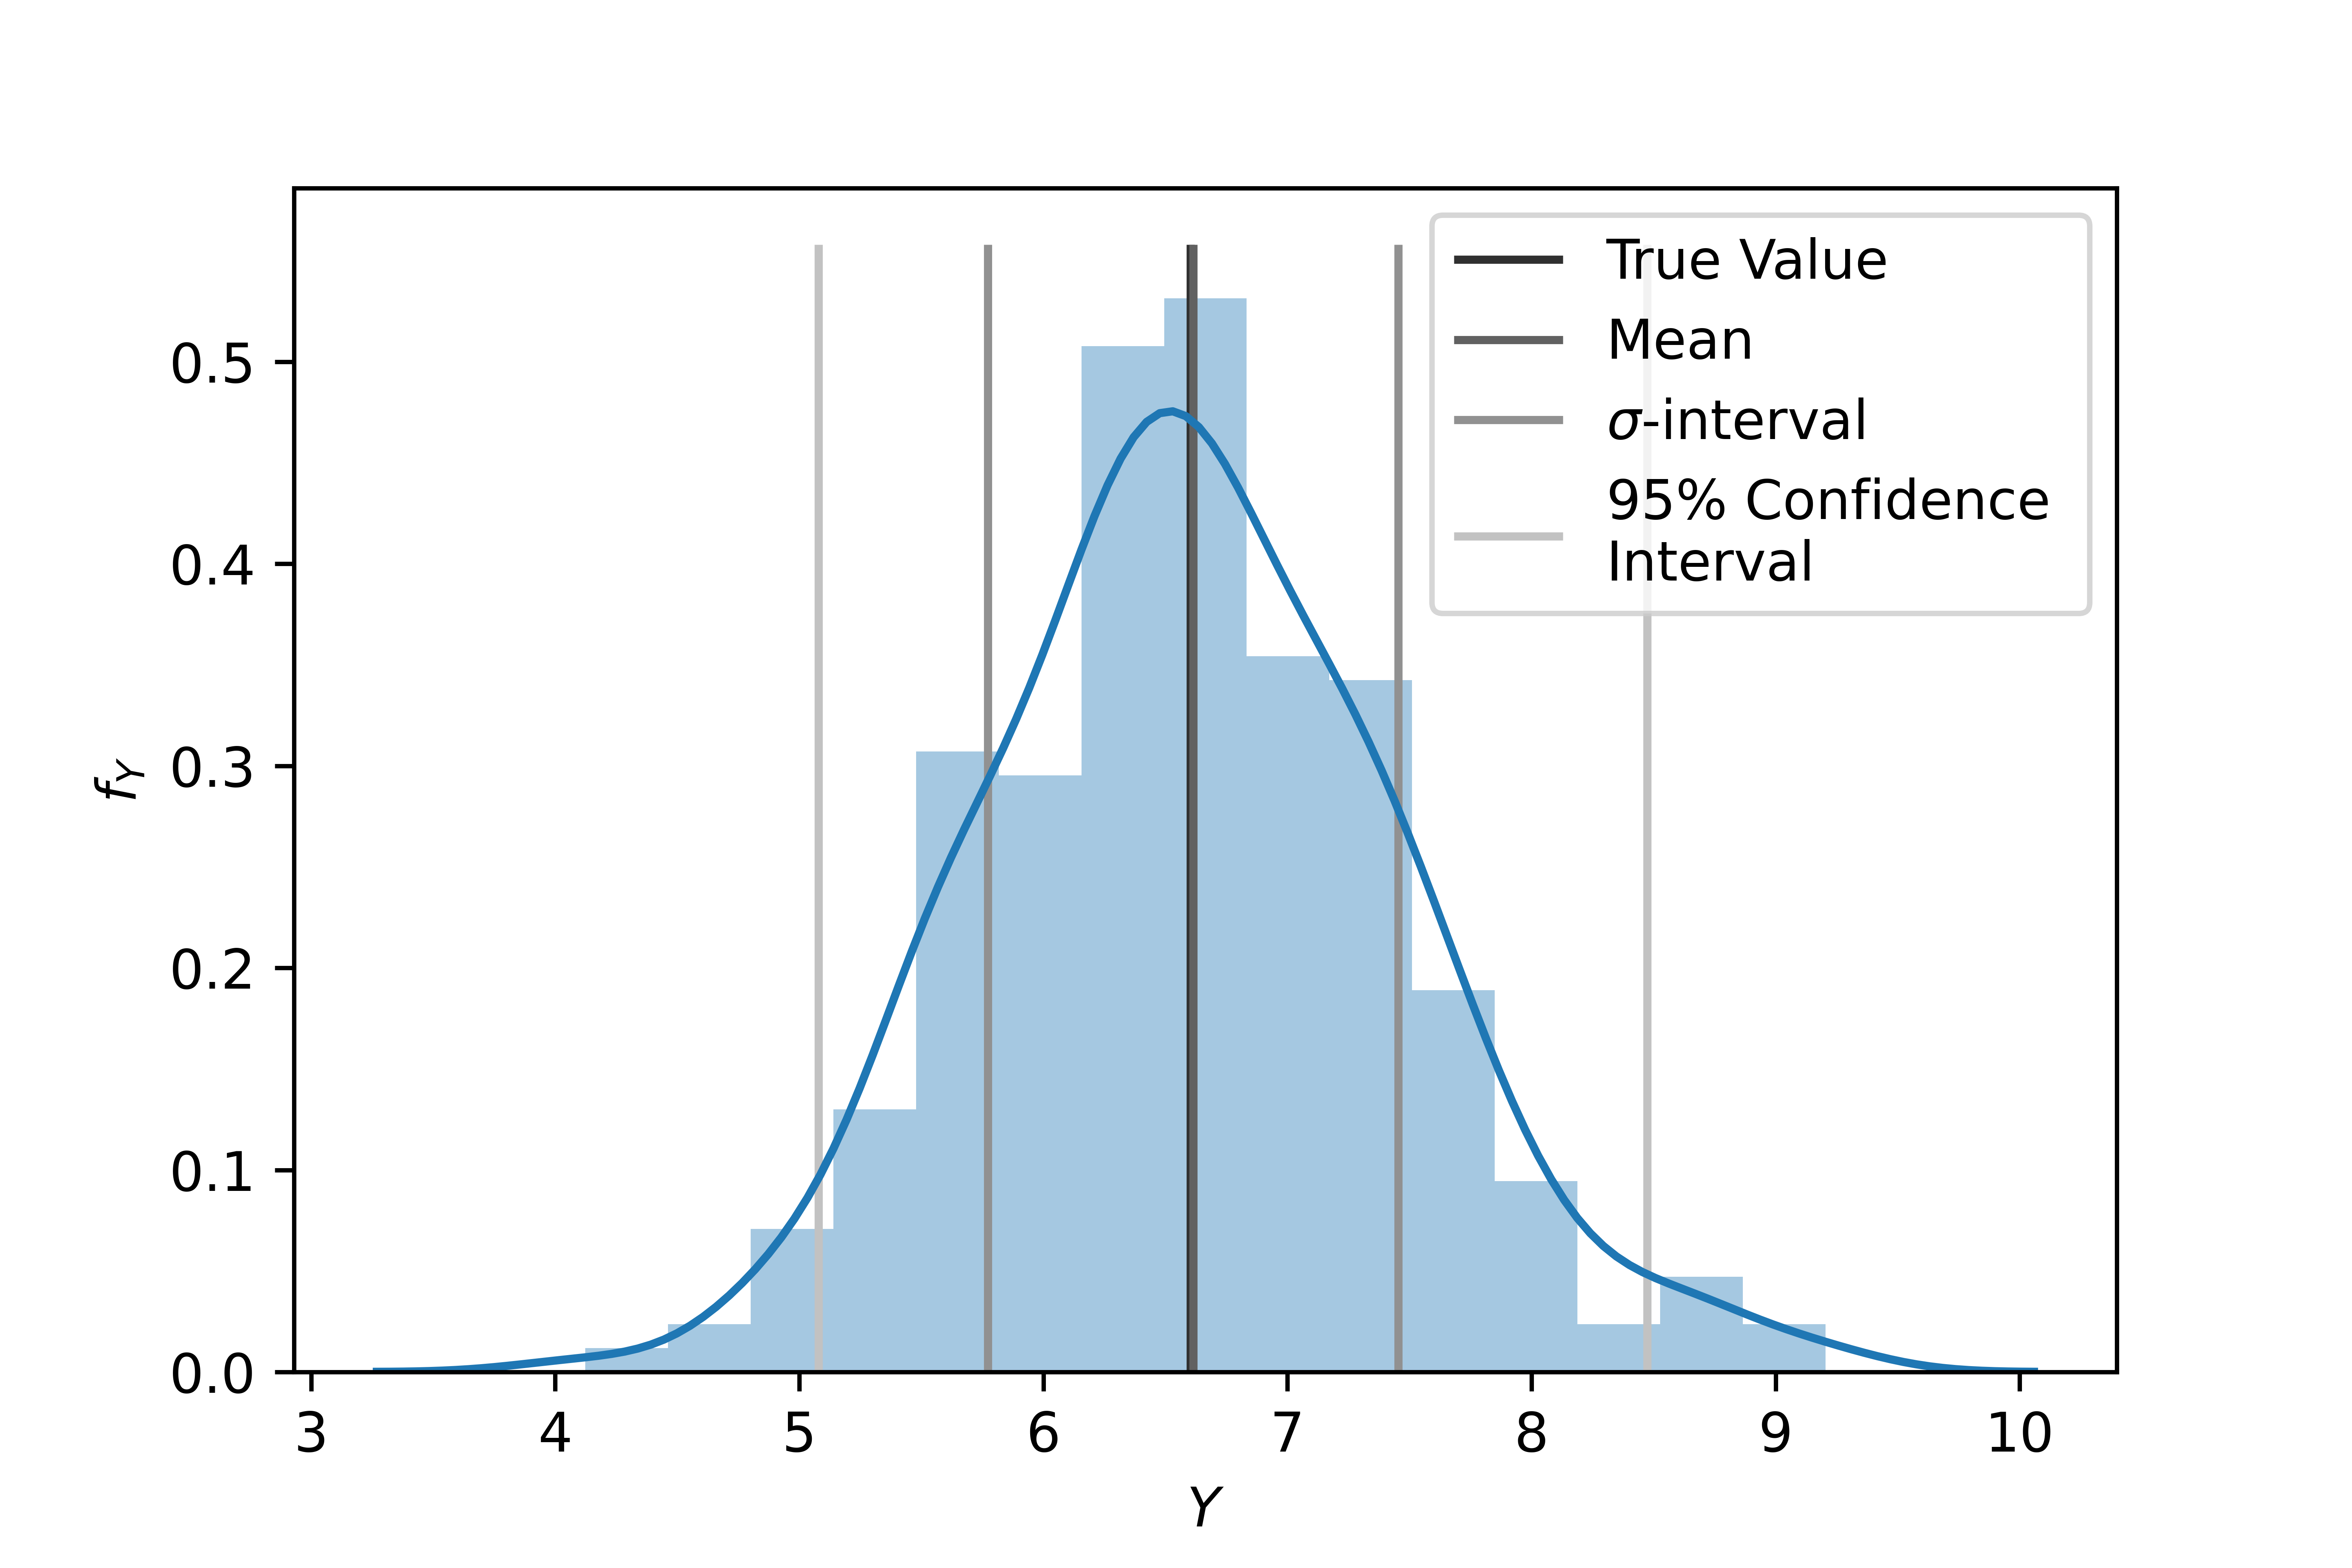
\includegraphics[scale=0.9]{../figures/figure_3.png}
	\label{figure3}
\end{figure}

We are now interested in how this paremeter uncertainty translates into uncertainty around some quantity of interest. For the remainder of this paper I am interested in how high expected annual demand for bus engines will be if the equilibrium price for engine replacement drops to 11,000 Dollars (as a reminder the cost function is scaled by 0.001 which means that the true $RC$ corresponds to 11,725.70 Dollars) and the bus fleet consists of 50 buses. In the language of the UQ framework the demand function in equation \ref{eq19} corresponds to the computation model $f(.)$ in equation \ref{compmodel} and \ref{uncertaincompmodel}. The propagation of the random vector $\Theta = (\hat{RC}, \hat\theta_{11}, \hat\theta_3)^{N=250}_n$ across the Monte Carlo runs results in the random vector $Y$ which equals to the expected annual demand at replacement costs of 11,000 Dollars. The uncertainty in the QoI $Y$ is depicted in Figure \ref{figure3}.


The calculated empirical mean of $Y$ across the Monte Carlo runs is very similar to the true expected demand (which is derived from the true parameter vector). The interval of one standard deviation around the mean ranges from around 5.8 to 7.5 while the 95\% bootstrap confidence interval stretches from 5.1 to 8.5.\footnote{The percentile bootstrap is used (compare \cite{Davison.1997} chapter 5).} This uncertainty obviously also translates into the view on the whole expected demand function across a range of different replacement costs. Figure \ref{figure4} below corresponds to the implied demand function in Figure 7 of \cite{Rust.1987} while being calculated for 50 buses and for the model setup of \cite{Iskhakov.2016}. To Rust's figure I now add uncertainty resulting from the calibration procedure. I obtain a well-behaved downward sloping demand function for which the mean across our Monte Carlo simulation corresponds closely to the true expected demand function.

This constitutes the end of the description on the basic idea of uncertainty quantification in the Rust Model. In the next sections, I will use this framework to vary other key specifications of the model and the calibration procedure to investigate how this translates into the uncertainty of the QoI described above and whether this might differ when using MPEC as opposed to the NFXP.

\begin{figure}[H]
	\caption{The Implied Demand Function accounting for Parameter Uncertainty}
	\vspace*{-4mm}
	\centering
	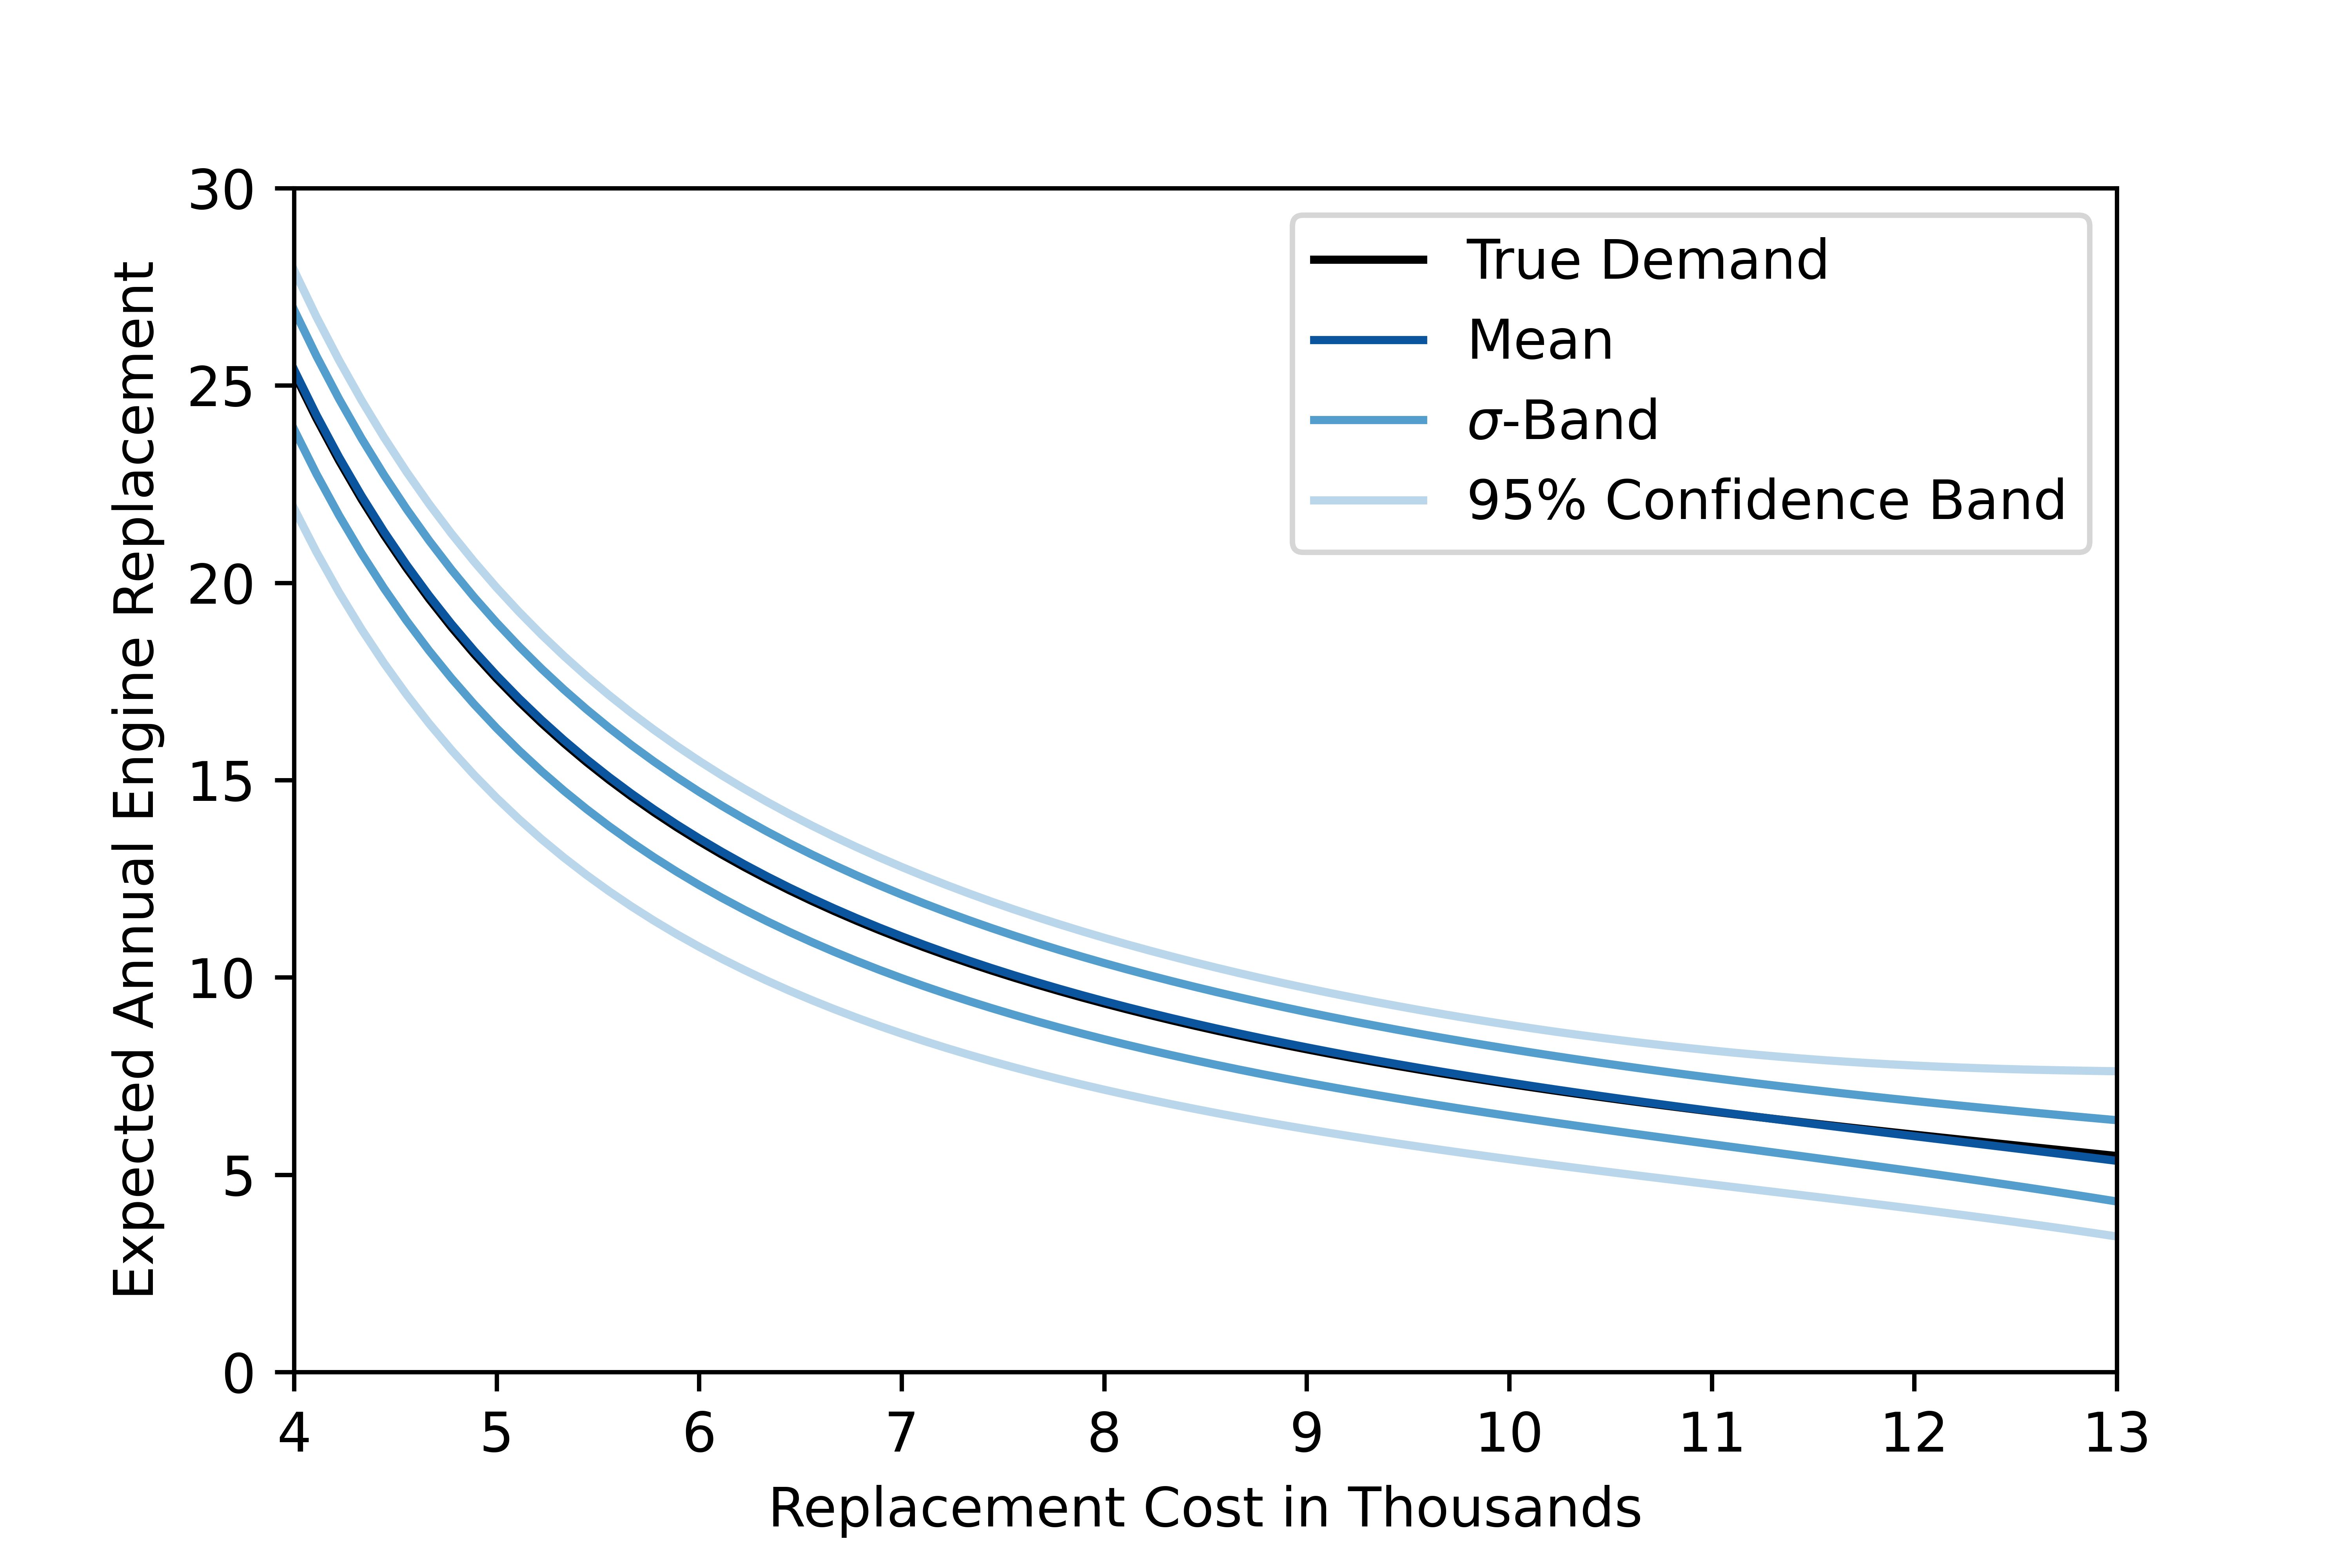
\includegraphics[scale=0.9]{../figures/figure_4.png}
	\label{figure4}
\end{figure}










\section{Sensitivity of the Rust Model}
\thispagestyle{plain} % surpress header on first page
% Resources
\newpage
\thispagestyle{plain} % no header on first page
\addcontentsline{toc}{section}{References} %toc steht für table of contents

\bibliography{bibliography/literature}

% Appendix
\newpage
\thispagestyle{plain} % no header on first page
\addcontentsline{toc}{section}{Appendix}

\chead{\textit{\nouppercase{Appendix}}}

\thispagestyle{plain} % surpress header on first page

\subsection{Appendix A} \label{appendixA}
\thispagestyle{plain} % surpress header on first page

This part explains to which extent my implementations of the NFXP and MPEC differ to the ones by \cite{Iskhakov.2016}. As already laid out in section \ref{generalsetup}, we rely entirely on open-source programs which has some implications for our methodology. The authors use matlab for the NFXP (they also implement the BHHH like this) and the modeling language AMPL in combination with the solver KNITRO for MPEC. I, on the other hand, implement everything in Python only and use IPOPT as a solver for MPEC. This alone can cause the their results and mine to differ. Additionally, for MPEC they obtain first and second order analytical derivatives of the Lagrangian as AMPL provides them using automatic differentiation. While there are tools such as JAX \footnote{See https://github.com/google/jax .} that provide analytical derivatives via automatic differentiation for code written in Python, these restrict the code to have a certain form which would have involved rewriting main parts of the existing code. This might be an interesting extension of the package for later but is out of bounds for this thesis. I decided therefore to at least code up the first order derivative by hand and pass it on to IPOPT. The fact that the Hessian has to be approximated can potentially influence the results strongly. \citeauthor{Iskhakov.2016} also give sparsity patterns of the two derivatives to KNITRO in order to conserve memory and increase speed. This is not done in my implementation. Another practical difference comes from the fact that KNITRO and IPOPT rely on different stopping criteria which makes it impossible to exactly replicate the setup for KNITRO with IPOPT. For the NFXP there are also some differences. My BHHH as well as the switching from contraction to N-K iterations has other tolerances. On top of that, \citeauthor{Iskhakov.2016} allow the fixed point algorithm to switch back from N-K to contraction steps when a certain criteria is met. This flexibility is not implemented in my code.

In the light of that, the algorithms by \citeauthor{Iskhakov.2016} are slightly more complex and robust which seems to affect the number of iterations and function evaluations for MPEC and especially the amount of contraction and N-K steps needed in the case of the NFXP. This can be observed in Table \ref{table1}. Although one should mention that the more comparable implementation of MPEC in which \cite{Su.Judd.2012} use matlab as the modeling language and KNITRO with only first order analytical derivatives as solver seems to be inferior to my implementation when looking at the number of iterations and function evaluations needed \footnote{To see this, have a look at Table II on page 2228 of \cite{Su.Judd.2012}. One has to be cautious, though, as their implementation differs from mine in the sense that they do not recenter the expected value function.}. For an additional sanity check I provide the mean and standard deviations of the estimated cost parameters across the Monte Carlo simulations outlined in section \ref{generalsetup}. These are meaningful as \cite{Su.Judd.2012} argue that this simulation actually constitutes a parametric bootstrap procedure. The two statistics are provided for both my implementations and additionally for the NFXP of \citeauthor{Iskhakov.2016}. These results were not published but had to be obtained by me using their matlab replication code. Unfortunately, their code does not run through but only did with some additional changes. This should make one a bit cautious regarding these results. All of those results are presented in the table below in which can be seen that apart from when $\beta$ equals $0.995$ the results of all three approaches are very similar. \paragraph{}

\begin{table}[H]
	\centering
	\caption{Comparison to the Results of Iskhakov et al. (2016)}
	\begin{tabular}{l c c c c}
		\toprule\midrule
		& & & RC & $\theta_{11}$ \\
		\cmidrule{4-5}
		$\beta$ & Implementation & True Values: & $\mathbf{11.726}$ & $\mathbf{2.457}$ \\ \midrule
		0.975 & MPEC & Mean & 11.908 & 2.507 \\
		& & Std. Dev. & (1.517) & (0.486) \\
		& NFXP & Mean & 11.908 & 2.507 \\
		& & Std. Dev. & (1.517) & (0.468) \\
		& NFXP Iskhakov & Mean & 11.914 & 2.508 \\
		& & Std. Dev. & (1.517) & (0.468) \\ \midrule
		0.985 & MPEC & Mean & 11.986 & 2.534 \\
		& & Std. Dev. & (1.457) & (0.452) \\
		& NFXP & Mean & 11.986 & 2.534 \\
		& & Std. Dev. & (1.457) & (0.452) \\
		& NFXP Iskhakov & Mean & 11.991 & 2.535 \\
		& & Std. Dev. & (1.457) & (0.452) \\ \midrule
		0.995 & MPEC & Mean & 11.891 & 2.508 \\
		& & Std. Dev. & (1.384) & (0.440) \\
		& NFXP & Mean & 11.891 & 2.508 \\
		& & Std. Dev. & (1.384) & (0.440) \\
		& NFXP Iskhakov & Mean & 11.191	& 2.902 \\
		& & Std. Dev. & (1.188) & (0.473) \\ \midrule
		0.999 & MPEC & Mean & 11.874 & 2.513 \\
		& & Std. Dev. & (1.347) & (0.444) \\
		& NFXP & Mean & 11.874 & 2.513 \\
		& & Std. Dev. & (1.347) & (0.444) \\
		& NFXP Iskhakov & Mean & 11.876	& 2.513 \\
		& & Std. Dev. & (1.346) & (0.444) \\ \midrule
		0.9995 & MPEC & Mean & 11.849 & 2.509 \\
		& & Std. Dev. & (1.343) & (0.445) \\
		& NFXP & Mean & 11.847 & 2.508 \\
		& & Std. Dev. & (1.343) & (0.445) \\
		& NFXP Iskhakov & Mean & 11.849 & 2.509 \\
		& & Std. Dev. & (1.342) & (0.445) \\ \midrule
		0.9999 & MPEC & Mean & 11.815 & 2.498 \\
		& & Std. Dev. & (1.319) & (0.431) \\
		& NFXP & Mean & 11.815 & 2.499 \\
		& & Std. Dev. & (1.319) & (0.431) \\
		& NFXP Iskhakov & Mean & 11.817	& 2.499 \\
		& & Std. Dev. & (1.319) & (0.431) \\ \bottomrule
	\end{tabular}
\end{table}

My implementations overestimate the true parameter slightly for $RC$ while coming gradually closer to the true value with increasing $\beta$. This pattern can also be seen in Table I of \cite{Su.Judd.2012} (who base their analysis on the same data generating process) which makes me confident that my results are correct. It seems like for $\beta = 0.995$ the NFXP Iskhakov is trapped in another local minimum that causes it to overestimate the true $\theta_{11}$ by a lot and suddenly underestimate the true $RC$. As mentioned before, this is likely to be caused by the fact that their code did not run through and it is not obviously clear whether the setup in the code is exactly like the one the published results are based on.

\newpage
\thispagestyle{empty} % e.g. no page number
\section*{Affidavit}
\vspace*{1.0cm}
"I  hereby confirm that the  work  presented  has  been  performed  and interpreted solely by myself except for where I explicitly identified the contrary. I assure that this work has not been presented in any other form for the fulfillment of any other degree or qualification. Ideas taken from other works in letter and in spirit are identified in every single case."\\
\newline
\newline
\newline

\noindent

\rule{5.5cm}{0.4pt} \phantom{ssssssssssssssssspace} \rule{5.5cm}{0.4pt}\\
\phantom{space}Place, Date \phantom{sssssssssssssssssssssssssssssssssssssspace} Signature



\end{document}
